%\documentclass[12pt]{article}
\documentclass[aip,jcp,preprint,superscriptaddress,floatfix]{revtex4-1}
\usepackage{url,graphicx,tabularx,array,geometry,amsmath,listings}
\setlength{\parskip}{2ex} %--skip lines between paragraphs
\setlength{\parindent}{20pt} %--don't indent paragraphs

\usepackage[colorinlistoftodos,prependcaption,textsize=tiny]{todonotes} %--TODO notes

\setlength{\headheight}{-50pt}
\setlength{\textheight}{700pt}
\setlength{\textwidth}{500pt}
\setlength{\oddsidemargin}{-10pt}
\setlength{\footskip}{50pt}
\usepackage{graphicx}% Include figure files
\usepackage{bm}
\usepackage{url}
\usepackage[colorlinks = true,
            linkcolor = blue,
            urlcolor  = blue,
            citecolor = blue,
            anchorcolor = blue]{hyperref}
\graphicspath{{./Figures/}}

%-- Commands for header
\renewcommand{\title}[1]{\textbf{\large{#1}}\\}
\renewcommand{\line}{\begin{tabularx}{\textwidth}{X>{\raggedleft}X}\hline\\\end{tabularx}\\[-0.5cm]}
\newcommand{\leftright}[2]{\begin{tabularx}{\textwidth}{X>{\raggedleft}X}#1%
& #2\\\end{tabularx}\\[-1cm]}

%\linespread{2} %-- Uncomment for Double Space
\begin{document}

\title{\center{Monte Carlo Simulation of the Lennard Jones Fluid in the Canonical Ensemble}}
\rule{\textwidth}{1pt}
\leftright{The Molecular Sciences Software Institute}{Eliseo Marin-Rimoldi and John D.~Chodera} %-- left and right positions in the header

\bigskip

\section{Introduction}
\subsection{Monte Carlo Integration}

In statistical mechanics, we are interested in computing averages of
thermodynamic properties as a function of atom positions and momenta~\cite{Tuckerman.Book,Hill.Book,McQuarrie.Book}.
A thermodynamic average depending only on configurational properties can be computed using the following
expectation value integral
\begin{equation}
	\left<Q\right> = \int_V Q\left(\textbf{r}^N\right)
	\rho\left(\textbf{r}^N\right) d\textbf{r}^N
	\label{eq.statMechAverage}
\end{equation}
$\textbf{r}^N$ is a $3N$ dimensional vector containing the positions of the $N$ atoms,
where $Q(\textbf{r}^N)$ is the thermodynamic quantity of interest that depends only on the configuration $\textbf{r}^N$, 
$\rho\left(\textbf{r}^N\right)$ is the probability
density whose functional form depends on the statistical mechanical ensemble
of interest, and $V$ defines the volume of configuration space over which $\rho$ has support. 
Note that the integrals over momenta have been factored out, as
they can be evaluated
analytically. The integral (Eq.~\ref{eq.statMechAverage}) is very hard to compute
even for small atomic systems.
For instance, a monoatomic system of 10 atoms leads to a 30-dimensional
integral. Consequently, we need to resort to a numerical integration scheme if we want to
study atomic systems.

Monte Carlo methods are numerical techniques
frequently used to estimate complex multidimensional
integrals which otherwise
 could not be performed~\cite{Liu.Book,Newman.Book}.
 For instance, the integral of the function $f(\textbf{x})$,
 where \textbf{x} is a higher-dimensional vector, is approximated as
 \begin{equation}
	 I = \int_V f(\textbf{x}) \, d\textbf{x} = \int_V
	 \frac{f(\textbf{x})}{h(\textbf{x})} h(\textbf{x}) \, d\textbf{x} 
	 = \left< \frac{f(\textbf{x})}{h(\textbf{x})} \right>_{h(\textbf{x})}
	 \label{eq.averageGeneral}
 \end{equation}
 The idea of Monte Carlo integration is to estimate the expectation value
 $\left<\frac{f(\textbf{x})}{h(\textbf{x})}\right>_{{h(\textbf{x})}}$ by
 generating random samples of \textbf{x} from the probability density $h(\textbf{x})$. 

\subsection{Importance Sampling}

In Equation \ref{eq.averageGeneral}, we are free to chose the probability
distribution
$h(\textbf{x})$. The simplest case is to uniformly generate $\textbf{x}$
in the volume $V$. In this way, $h(\textbf{x})$ becomes constant as
\begin{equation}
	h(\textbf{x}) = \frac{1}{V}
	\label{eq.uniformDist}
\end{equation}
Using this sampling density $h(\textbf{x})$, the integral (Eq.~\ref{eq.averageGeneral}) becomes
\begin{equation}
	I = \int_V f(\textbf{x}) \, d\textbf{x} \approx \frac{V}{N} \sum_{i=1}^N
	f(\textbf{x}_i)
	\label{eq.averageUniform}
\end{equation}
where N is the total number of random samples and $f(\textbf{x}_i)$ is the
integrand evaluated using the $i^{th}$ sample. While using a
uniform sampling density often works sufficiently well for simple unidimensional cases, it generally fails to produce useful estimates
for complex problems.

The problem at hand involves the evaluation of $N$-dimensional
integral \ref{eq.statMechAverage}, which is dominated by a small region of configuration space~\cite{Tuckerman.Book,Hill.Book,McQuarrie.Book}. 
Using a uniform probability distribution $h(\textbf{r}^N)$ to generate
representative samples of this subset is not efficient,
as most states generated this way would have a low weight.

A solution to this problem is to generate positions $\textbf{r}^N$ according to
the distribution $\rho\left(\textbf{r}^N\right)$. This is a way to generate
relevant configurations more frequently than configurations that have low
probability.
Mathematically, we set $h(\textbf{r}^N)=\rho\left(\textbf{r}^N\right)$.
This idea is known as \textit{importance sampling}.

Combining Eqs.~\ref{eq.statMechAverage} and \ref{eq.averageGeneral}
and the condition $h(\textbf{r}^N)=\rho\left(\textbf{r}^N\right)$,
we find that
\begin{equation}
	%\left<Q\right> = \frac{\int Q e^{-\beta U\left(\textbf{r}^N\right)}
	%d\textbf{r}^N}{\int e^{-\beta U\left(\textbf{r}^N\right)}
	%d\textbf{r}^N}
	\left<Q\right> \approx \frac{1}{N} \sum_{i=1}^N Q\left(\textbf{r}_i^N\right) .
	\label{eq.importanceSamplingAverage}
\end{equation}
Thus, we can get thermodynamic properties by simply computing an arithmetic
average, given
that we perform importance sampling from $h(\textbf{r}^N)=\rho\left(\textbf{r}^N\right)$.

\subsection{Detailed Balance Condition}

The question now becomes how to generate such atomic positions $\textbf{r}^N$
(or \textit{states}) distributed
according to $\rho\left(\textbf{r}^N\right)$. In 1953, Metropolis, Rosenbluth, Rosenbluth, and Teller introduced a
solution based on Markov chains~\cite{Metropolis.JCP.21.1087.1953}. 
They proposed to use the detailed balance
condition in order to ensure proper configurational sampling from
the statistical mechanical distribution of interest. In order to generate
a new configuration $n$ from an old configuration $m$,
the detailed balance condition is

\begin{equation}
	\rho_m\left(\textbf{r}^N\right) \alpha \left(m \rightarrow n \right)
	P_{acc} \left(m \rightarrow n \right) =
	\rho_n\left(\textbf{r}^N\right) \alpha \left(n \rightarrow m \right)
	P_{acc} \left(n \rightarrow m \right) 
	   \label{eq.detailedBalance}
\end{equation}

Where $\rho_m\left(\textbf{r}^N\right)$ is the probability of observing
state $m$,
$\alpha \left(m \rightarrow n \right)$ is the probability of
attempting to generate a new state $n$ starting from a state $m$  and 
$P_{acc} \left(n \rightarrow m \right)$ is the probability of accepting 
such transition. Basically, the condition of detailed balance tells us that the
``flux'' of transitions
from state $m$ to state $n$ equals the flux from state $n$ to state $m$ at
equilibrium.

There are many ways to satisfy Eq.~\ref{eq.detailedBalance}. 
Metropolis et al.\ suggested to use the $min$ function as
\begin{equation}
	P_{acc}(m \rightarrow n) = \text{min} \left[1,\frac{\alpha \left(n
		\rightarrow m \right)}{\alpha \left(m \rightarrow n \right)}
		\frac{\rho_n\left(\textbf{r}^N\right)}{\rho_m\left(\textbf{r}^N\right)}
	\right]
	\label{eq.detailedBalanceFinal}
\end{equation}

\section{Canonical Ensemble Monte Carlo of a Lennard Jones Fluid}

Assume we have $N$ monoatomic particles that interact using the Lennard-Jones (LJ) potential:
\begin{equation}
U\left(r_{ij} \right) = 4 \epsilon \left[\left(\frac{\sigma}{r_{ij}}\right)^{12} -\left(\frac{\sigma}{r_{ij}}\right)^{6} \right]
\end{equation}
where $r$ is the interparticle distance, $\sigma$ is the distance where the interaction energy is zero, and $\epsilon$ is the well depth. 
\todo[inline]{We will want to add a switching function $S(r)$ with continuous first and second derivatives or else we' are going to run into issues with molecular dynamics integrators, energy conservation, and large errors in configuration space sampling.} 

Our goal is to generate a set of states of $N$ LJ particles distributed according to the canonical (NVT) ensemble
\begin{eqnarray}
	\rho_n \left(\textbf{r}^N ; \beta \right) &=& Z(\beta)^{-1} e^{-\beta U \left( \textbf{r}^N \right)} \label{eq:nvtDist} \\
	Z(\beta) &\equiv& \int_V e^{-\beta U \left(  \textbf{r}^N \right)} \, d\textbf{r}^N 
\end{eqnarray}
where $U \left( \textbf{r}^N \right)$ is the potential energy of the system, $\beta = (k_B T)^{-1}$ is the inverse temperature, $k_B$ is the Boltzmann constant, and $T$ is the absolute temperature. 

Note that  $U \left( \textbf{r}^N \right)$ is given by
\begin{equation}
	U \left( \textbf{r}^N \right) = \sum_{i < j} U \left( r_{ij} \right)
\end{equation}
Substituting Eq.~\ref{eq:nvtDist} into Eq.~\ref{eq.detailedBalanceFinal} and assuming $\alpha \left( n \rightarrow m \right) =  \alpha \left( m \rightarrow n \right)$, we obtain
\begin{equation}
	P_{acc}(m \rightarrow n) = \text{min} \left[
		1,e^{-\beta \Delta U}
	\right]
	\label{eq.detailedBalanceNVT}
\end{equation}

Where $\Delta U$ is the difference in potential energy of the system
between the new state $n$ and the old state $m$. Note that the argument
of the energy $\textbf{r}^N$ has been dropped for clarity.

\subsection{Flow of the Calculations in Metropolis Monte Carlo}

The following workflow can be used to implement the Metropolis algorithm to sample the canonical ensemble of configurations of LJ particles \cite{Shell.Notes, Maginn.Notes}:

\begin{enumerate}
\item Generate an inital system state $m$.
\item Choose an atom with uniform probability from $\{1, \ldots, N\}$ from old state $m$.
\item Propose a new state $n$ by translating a LJ particle by a uniform random displacement $\Delta x \sim U(-\delta, +\delta)$.
	%We will use a Gaussian displacement $\Delta x \sim \mathcal{N}(0, \delta^2)$, where $\delta$ is the standard deviation of the Gaussian displacement.
	\todo[inline]{Should this be uniform or Gaussian?}
	The displacement scale $\delta$ should not be too large as this would
	likely result in particle overlaps, but should not be too small
	as this would result in a slow sampling of configurational space.
	More on this below.
\item The difference in energy between the new and old states is computed.
\item The new state is accepted or rejected using the Metropolis criterion.
	Practically, this can be implemented as follows. 
	If a move from $m$ to $n$ is ``downhill'', $\Delta U \leq 0$,
	the move is always accepted. For ``uphill'' moves, a random
	number $\zeta$ is generated uniformly on (0,1).  
	If $\zeta < \exp[-\beta {\Delta U}]$, the move is
	accepted.  Otherwise, the move is rejected. 
	\todo[inline]{This will need to be modified for Gaussian displacement proposals.}
\end{enumerate}

\subsection{Technical considerations}

\textbf{Starting Configuration.} We
know that the final result should be independent of the starting
configuration, but from a practical standpoint, we have to start someplace. 
For this particular example, a good way to start is to place atoms
in a lattice. By performing translation moves, the lattice will ``melt''
and liquid configurations will be obtained. During this ``melting'' process, 
we do not take averages of thermodynamic properties, as we would be 
``equilibrating'' the system.
Once a configuration has been generated and a simulation run, you
can always use a ``snapshot'' from this simulation as a starting point for a
new configuration, as long as the conditions are similar.

\textbf{Equilibration.} To check whether the system has reached equilibrium, we 
monitor the potential energy and pressure.  We look for 
no systematic drift in either quantity, only 
fluctuations about a mean. This is usually achieved within ~1000N
translations attempts (or Monte Carlo steps) for low molecular weight
systems.

\textbf{Maximum displacement.} As mentioned before, part of the ``recipe''
of this method is translating a LJ particle by a random amount. This
displacement should not be too large as this would resulte in particle overlaps. It also should not be too small, as this would result in unefficient sampling.
A common practice is that the maximum particle displacement is adjusted
to achieve 50\% acceptance translation rates. 

\textbf{Energy truncation and tail corrections.} If two particles are separated
by more than a certain distance, we typically truncate their interaction energy if $r > r_c$, where $r_c$ denotes the \emph{cutoff distance}. 
Truncating interactions removes contribution to the potential energy that might be non negligible and can lead to significant artifacts, such as significantly perturbed densities when a barostat is used to sample the NPT ensemble due to neglected long-range dispersion interactions. 
We can estimate the truncated interactions by incorporating an energy 
correction, known as the tail or long range correction.
For the Lennard-Jones fluid, we assume that we have an homogeneous liquid at $r>r_c$ to obtain the correction for neglecting this contribution for all interacting pairs of particles:
\begin{equation}
	U_{tail} = \frac{8 \pi N^2}{3 V} \epsilon \sigma^3
	\left[\frac{1}{3} \left(\frac{\sigma}{r_c} \right)^9 
	- \left(\frac{\sigma}{r_c} \right)^3 \right]
\end{equation}
\todo[inline]{This will have to be modified if we use a switching function $S(r)$ in the potential.}

\textbf{System size and periodic boundary conditions.} A typical molecular 
simulation is carried out anywhere from 
10 to 10,000 particles. This amount of particles is far away of being
representative of a bulk liquid. To get around this problem, we employ a trick
called
periodic boundary conditions. The primary simulation box is surrounded
by copy images of itself. For a cubic simulation, there would be 26 
images around the central box. This trick has two implications
\begin{enumerate}
	\item If the position of a particle (i.e. Cartesian coordinates) is
		outside the simulation box after a particle translation, 
		an identical particle should enter the box through the
		opposite face of the box, as shown in Figure ~\ref{fig:pbc}.
	\item When measuring distances used in the evaluation of the LJ
		potential, we should measure the \textit{minimum
		image}. See Figure ~\ref{fig:minimumImage}.
\end{enumerate}

\begin{figure}[t]
	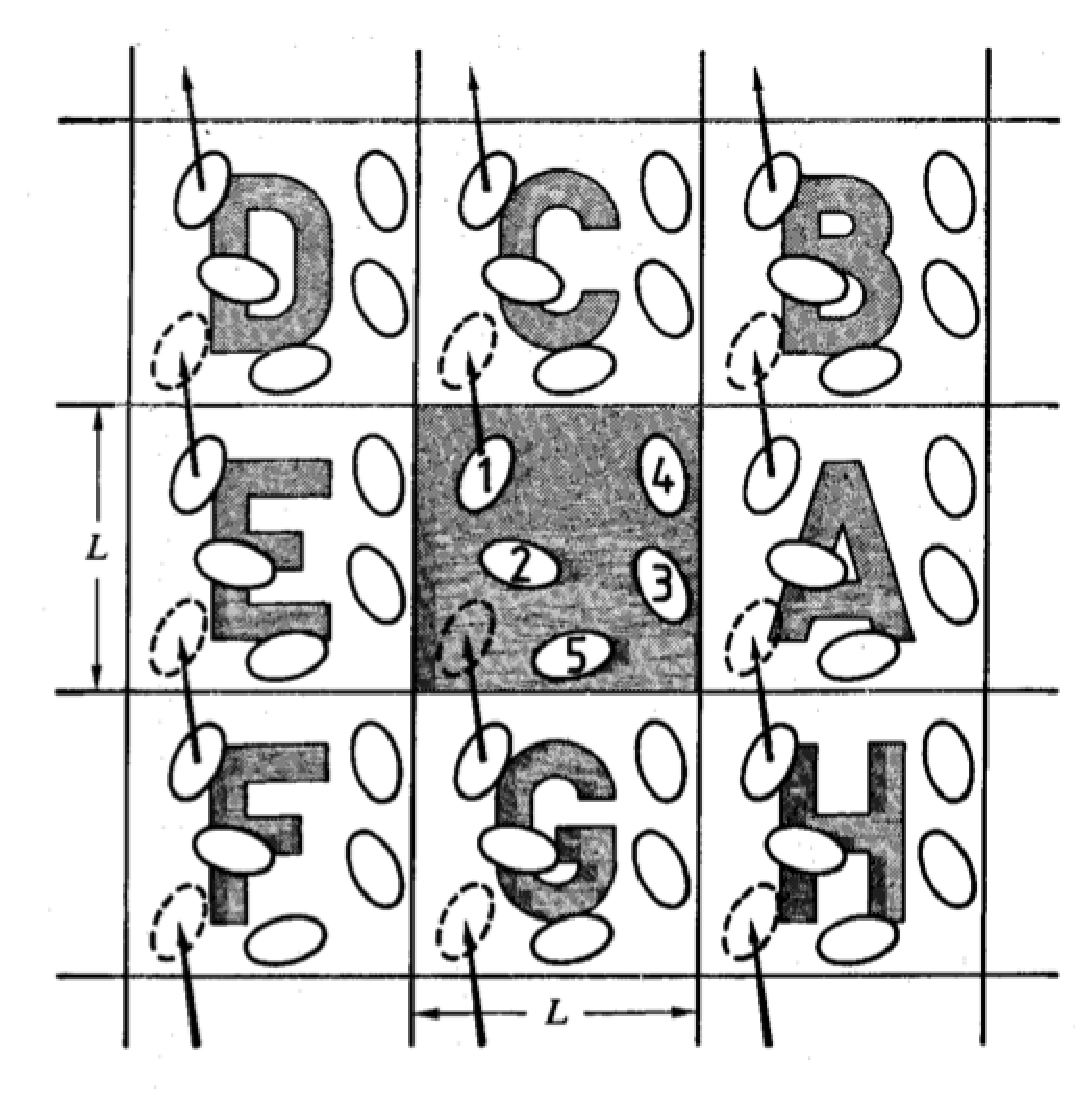
\includegraphics[scale = 0.5]{pbc.eps}
	\caption{Molecule one is displaced outside the bounds of the central box and placed back
	in through the oposite side of the box. Image from Allen and Tildesley. ~\cite{Allen.Book}}
	\centering
	\label{fig:pbc}
\end{figure}

\begin{figure}[t]
	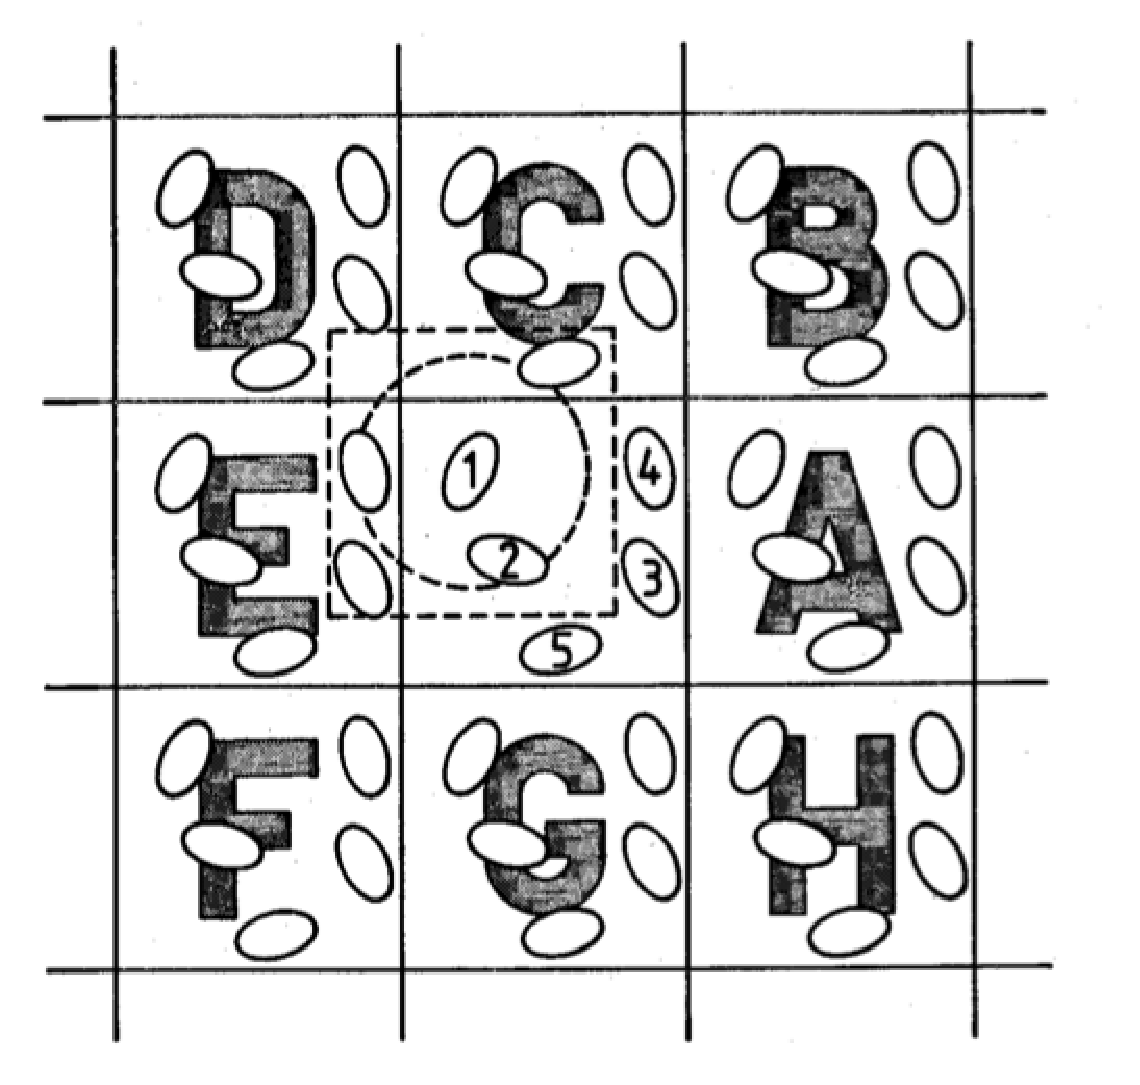
\includegraphics[scale = 0.5]{minimumImage.eps}
	\caption{Representation of the minimum image distance. Molecule 1 does not interact with 
		molecule 4 located in the simulation box because the distance between particles is 
		greater than the cutoff. However, molecule 1 does interact with
		the image of molecule 4 located in box E. Image from Allen and 
		Tildesley ~\cite{Allen.Book}}
	\centering
	\label{fig:minimumImage}
\end{figure}

\textbf{Pressure, the virial and pressure tail corrections.} To compute the system pressure, 
we use the virial theorem

\begin{equation}
	P = \frac{1}{3V} \left< 3 N k_B T + \sum_{i < j} \textbf{f}_i \cdot \textbf{r}_i  \right>
\end{equation}

Where 

\begin{equation}
	\sum_{i < j} \textbf{f}_i \cdot \textbf{r}_i = - \sum_{i < j} \frac{dU\left(r_{ij} \right)}{dr} r_{ij} = W
\end{equation}

The term $W$ is known as the virial and it is a pairwise sum and it can be computed 
alongside the energies. Note that the negative derivative of the energy is the force. 
For the LJ potential, this is

\begin{equation}
	\mathbf{f}\left(r_{ij} \right) = -\frac{dU \left(r_{ij} \right)}{dr} = - \frac{48 \epsilon}{r^2_{ij}} \left[\left(\frac{\sigma}{r_{ij}}\right)^{12} -\frac{1}{2}\left(\frac{\sigma}{r_{ij}}\right)^{6} \right] \mathbf{r}_{ij}
\end{equation}

The effect of the truncation of the interactions must be also taken into account for the pressure
computation using a correction term

\begin{equation}
	P_{tail} = \frac{16 \pi N^2}{3 V^2} \epsilon \sigma^3
	\left[\frac{2}{3} \left(\frac{\sigma}{r_c} \right)^9 
	- \left(\frac{\sigma}{r_c} \right)^3 \right]
\end{equation}
\todo[inline]{This will have to be modified if we use a switching function $S(r)$ in the potential.}

\textbf{Reduced Units.} You can render the LJ potential dimensionless as

\begin{equation}
	U^*\left(r_{ij} \right) = 4 \left[\left(\frac{1}{r^*_{ij}}\right)^{12} -\left(\frac{1}{r^*_{ij}}\right)^{6} \right]
\end{equation}

where 

\begin{equation}
	U^* = \frac{U}{\epsilon}
\end{equation}

and 

\begin{equation}
	r^* = \frac{r}{\sigma}
\end{equation}

This enables us to run a simulation using a ``generic'' LJ model and easily extract properties at different
conditions by simply multiplying by the appropriate factors (see Table \ref{table:reducedUnits}). 

\begin{table}[t]
\centering
 \begin{tabular}{|c c|} 
 \hline
 Quantity & Expression \\ [0.5ex] 
 \hline\hline
 Length &  $L^*=L / \sigma$   \\ 
 Density &  $\rho^* = N \sigma^3 / V$   \\
 Energy &  $U^* = U / \epsilon$   \\
 Pressure &  $P^* = P \sigma^3 / \epsilon$   \\
 \hline
 \end{tabular}
 \caption{Conversion factors between real and reduced units.}
 \label{table:reducedUnits}
\end{table}

\subsection{Reference calculations}

See the following resources for reference data:

\begin{itemize}
\item \href{https://mmlapps.nist.gov/srs/LJ_PURE/mc.htm}{NIST LJ reference}
\item \href{https://www.nist.gov/mml/csd/chemical-informatics-research-group/lennard-jones-fluid-reference-calculations}{LJ Energy states}
\end{itemize}

\newpage
%
\bibliographystyle{aip.bst}
\bibliography{references.bib}

\end{document}
